%; whizzy chapter
% -initex iniptex -latex platex -format platex -bibtex jbibtex -fmt fmt
% 以上 whizzytex を使用する場合の設定。


%     Tokyo Debian Meeting resources
%     Copyright (C) 2008 Junichi Uekawa

%     This program is free software; you can redistribute it and/or modify
%     it under the terms of the GNU General Public License as published by
%     the Free Software Foundation; either version 2 of the License, or
%     (at your option) any later version.

%     This program is distributed in the hope that it will be useful,
%     but WITHOUT ANY WARRANTY; without even the implied warranty of
%     MERCHANTABILITY or FITNESS FOR A PARTICULAR PURPOSE.  See the
%     GNU General Public License for more details.

%     You should have received a copy of the GNU General Public License
%     along with this program; if not, write to the Free Software
%     Foundation, Inc., 51 Franklin St, Fifth Floor, Boston, MA  02110-1301 USA

%  preview (shell-command (concat "evince " (replace-regexp-in-string "tex$" "pdf"(buffer-file-name)) "&"))
% 画像ファイルを処理するためにはebbを利用してboundingboxを作成。
%(shell-command "cd image200801; ebb *.png")

%%ここからヘッダ開始。

\documentclass[mingoth,a4paper]{jsarticle}
\usepackage{monthlyreport}

% 日付を定義する、毎月変わります。
\newcommand{\debmtgyear}{2008}
\newcommand{\debmtgmonth}{1}
\newcommand{\debmtgdate}{19}
\newcommand{\debmtgnumber}{36}

\begin{document}

\begin{titlepage}
\thispagestyle{empty}

% タイトルページ:編集必要な部分は最初のマクロに飛ばすこと

\vspace*{-2cm}
第\debmtgnumber{}回 東京エリア Debian 勉強会資料

\hspace*{-2.4cm}
\includegraphics[width=210mm]{image200801/2008title.eps}\\
\hfill{}\debmtgyear{}年\debmtgmonth{}月\debmtgdate{}日

\end{titlepage}

\dancersection{Introduction}{上川 純一}
 
 今月のDebian勉強会へようこそ。これからDebianの世界にあしを踏み入れると
 いう方も、すでにどっぷりとつかっているという方も、月に一回Debianについ
 て語りませんか?

 Debian勉強会の目的は下記です。

\begin{itemize}
 \item \underline{Debian Developer} (開発者)の育成。
 \item 日本語での「\underline{開発に関する情報}」を整理してまとめ、アップデートする。
 \item \underline{場}の提供。
 \begin{itemize}
  \item 普段ばらばらな場所にいる人々が face-to-face で出会える場を提供
	する。
  \item Debian のためになることを語る場を提供する。
  \item Debianについて語る場を提供する。
 \end{itemize}
\end{itemize}		

 Debianの勉強会ということで究極的には参加者全員がDebian Packageをがりがり
 と作るスーパーハッカーになった姿を妄想しています。

 情報の共有・活用を通して Debianの今後の能動的な展開への土台として、「場」
としての空間を提供するのが目的です。

\includegraphics[width=1\hsize]{image200712/debianmeetinganddebianjp.eps}

\newpage

\begin{minipage}[b]{0.2\hsize}
 \definecolor{titleback}{gray}{0.9}
 \colorbox{titleback}{\rotatebox{90}{\fontsize{80}{80} {\gt デビアン勉強会} }}
\end{minipage}
\begin{minipage}[b]{0.8\hsize}
\hrule
\vspace{2mm}
\hrule
\tableofcontents
\vspace{2mm}
\hrule
\end{minipage}

\dancersection{事前課題}{上川 純一}

今回の事前課題は以下です。

\begin{enumerate}
 \item 「こんなDebianパッケージを作成してみました・作成してみようとして
       みたらここまでしかできませんでした」\\
       2008年のDebian勉強会はDebianパッケージ作成について連続して企画を
       する予定です。現在どれくらいできるものなのか、どこらへんでつまっ
       ているのかを教えてください。(200-800文字)

 \item 「2008年のDebianの目玉を大胆に予想する」\\ 2008 年にどういう事が
       Debianの目玉になるのか、大胆に予想してみてください。
       (200-800文字)
\end{enumerate}

この課題に対して提出いただいた内容は以下です。

\subsection{吉田@板橋}

\subsubsection{「こんなDebianパッケージを作成してみました・作成してみようとしてみたらこ
こまでしかできませんでした」}
私は、たまに必要があると野良パッケージを作っています。
野良パッケージを作る理由としては、
\begin{enumerate}
 \item 	 使いたいアプリ/機能が公式パッケージにないから
 \item	 複数マシンにインストールしたり、環境再構築時に楽だから
 \item	 新規パッケージはstatbleに入らないから
 \item	 その他
\end{enumerate}
といったところです。
基本的には私のレベルは dh\_make して s で作るだけのレベルです。
その程度ですが、某LUGで入門として話してみたことがあります。
deb作成はrpm作成と比べて作業や決まり事が多くて少し面倒とおもいます。
が、仕事で作っていたrpmに比べて、
まだdebを作り慣れていないせいも多いと思います。

\subsubsection{「2008年のDebianの目玉を大胆に予想する」}
lennyリリース!というのは皆書きそうなので...
某社からDebianプリインストール機が出る...とか
あると面白いですね(笑)。

\subsection{日比野 啓}

\subsubsection{こんなDebianパッケージを作成してみました}

仕事でも趣味でも必要があれば自分でもパッケージングをやってます。
debianディレクトリのテンプレートは、perlならdh-make-perlを、そうでなければdh\_makeを使っています。
ビルドはdebuildでlintianでチェックしています。
perlモジュールのNet::SSH::Perlのパッケージングを仕事でやったときが一番大変でした。
(sshをperlで実装してあるため、大量の依存モジュールが^^;)
Cのヘッダの型情報と動的ライブラリを使ってCの関数をSchemeの処理系であるgaucheから呼び出すc-wrapperライブラリとか、
Cのソースコードを解析してObjective Camlの抽象木にしてくれるcilライブラリとかを趣味でパッケージングしました。

\subsubsection{小ネタ: 2008年のDebianの目玉を大胆に予想する}

experimentalにはもう有るようですが perl-5.10 あたりでしょうか。
ぜんぜん大胆じゃない^^;
pythonとperlが両方ともparrotの上に乗るとか。


\subsection{山本}

\subsubsection{「こんなDebianパッケージを作成してみました・作成してみようとしてみたらこ
こまでしかできませんでした」}
タールボールから野良ビルドする時は、必ずパッケージにすることにしています。
ただ、パッケージを2つ以上に分割する方法は、見様見まねで、よくわかってい
ません。
あと、新しいポリシー (3.7.3) の変更点もいまいち理解できていないと思います。

\subsubsection{「2008年のDebianの目玉を大胆に予想する」}

lenny フリーズ!
リリースは再来年に持ち越し!


\subsection{山根}


\subsubsection{「こんなDebianパッケージを作成してみました・作成してみようとしてみたらここまでしかできませんでした」}

\begin{itemize}
 
 \item  JD という 2ch ブラウザをパッケージに。パッケージとしてはあまりいじらなくても良い状態になっています。upstream が活発なのでそれに併せて更新予定です。
 \item  eclipse-nls-sdk は、upstream が音沙汰無いのでどうしたものか。分割方法を考えた方がいいのが課題。とりあえず lintian の warning だけ何とかします。そう言えば今思い出しましたが、Pleiades をパッケージ化できないかを upstream な人に KOF で尋ねられていたのでした。すっかり忘れてた。これも検討しないといかんですね。
 \item  ccspatch (linux-patch-tomoyo)、ccstools (tomoyo-ccstools) については一段落しました。backports を作って、upstream に利用を明示する必要がありそうです。
 \item  mirmon というパッケージを作って ITP しましたが、mentors でスポンサーしてあげるよといった DD がそれっきり音沙汰無いのでどうしたものかと思っています。delel@jp で聞くべきかも。
 \item  フォントパッケージを増やしています。ttf-vlgothic、ttf-konatu、
	ttf-kiloji が今まで accepted。次は ttf-togoshi-gothic、ttf-ume
	が手元では出来ているので、細かな所を upstream に確認ののち、ITP
	→upload 予定。確認出来ているフリーなフォントはどんどん追加予定です。
 \item  sylph-searcher をパッケージにしたいな、と思ったのですが、libsylph を作らないといけないのですね。library package は今のところ作って無いのでどうしたものか。
\end{itemize}

 すでにパッケージを upload した人は、lintian.debian.org で自分のパッケージの warning を確認してどんどん潰すべきですな


\subsection{前田 耕平}


\subsubsection{「こんなDebianパッケージを作成してみました・作成してみようとしてみたらこ
こまでしかできませんでした」}

年末年始でようやく一部のサーバをEtch化し始めました。ついでに自宅環境で使っているスクリプトの配布には、Debianパッケージにしてみようか、と思ったわけですね。で、じゃあスクリプトだけをパッケージ化するのはどうやるのかと、調べようとする前に、scpで転送してしまい、やらずじまいでした…。orz
何かのついでに始めてみようというのは、ダメですね…。今度の日曜(今月のDebian勉強会の翌日)ちゃんと時間を割いてやります。

\subsubsection{「2008年のDebianの目玉を大胆に予想する」}

きっと誰かがWiiもDebianにして、Wii Balance BoardでAPTシェルを自由自在に操っているに違いない。w

\subsection{岩松信洋}


\subsubsection{こんなDebianパッケージを作成してみました
  作成してみようとしてみたらここまでしかできませんでした}

最近作ったDebianパッケージは
\begin{itemize}
 \item  Macbook のLEDを Ethernetのアクセスに合わせて点灯させるソフトウェア
 \item  u-boot 用のイメージを作成するソフトウェア
\end{itemize}
です。

両方ともDebianパッケージ化を行い、手元で使っています。
パッケージ化がむずかしいソフトウェアではないので、特にハマることは
ありませんでした。

なので、いじられるところは特にありません。


\subsection{Noriaki Sato}

以前、Ruby on Rails で Oracle を使うために
ruby-oci8 を install しようとしたら deb package が無かったので、
package を作ってみようとした事がありました。
\url{http://www.debian.org/doc/manuals/maint-guide/index.ja.html#contents}
辺り(古い?)を斜め読みしながらやったのですが、
\begin{commandline}
 $ dpkg-buildpackage -r fakeroot
\end{commandline}
した所で、何故か /usr/local 配下に install されてしまいました。
その時は、普通に install したのと同じ結果になっただけなので、
まあいっか、とゆー事で終わりにしてしまったのですが、
良い機会なので少し調べてみました。
\begin{commandline}
 
 $ tar xvfz ruby-oci8-1.0.0.tar.gz
 $ cd ruby-oci8-1.0.0
 $ dh_make -e mail_address -f ruby-oci8-1.0.0.tar.gz
 $ dpkg-buildpackage -r fakeroot
 (snip)
 dh_installdirs
 # Add here commands to install the package into debian/tmp
 /usr/bin/make DESTDIR=/home/noriaki/tmp/deb/ruby-oci8-1.0.0/debian/tmp install
 make[1]: ディレクトリ `/home/noriaki/tmp/deb/ruby-oci8-1.0.0' に入ります
 ruby setup.rb install
 ---> lib
 mkdir -p /usr/local/lib/site_ruby/1.8/
 install oci8.rb /usr/local/lib/site_ruby/1.8/
 Permission denied - /usr/local/lib/site_ruby/1.8/oci8.rb
 Try 'ruby setup.rb --help' for detailed usage.
\end{commandline}
ということで、いまさら Makefile を眺めてみた所、
そもそも DESTDIR がなく、install 先が簡単に変更出来ない感じでした。
Makefile から呼び出している setup.rb という script を読んで、
Makefile を書き換えないとダメっぽいです。
今回は時間がなく、ここまでで断念しました。
そもそも、package の作り方はまだ良く分かっていない所が多いので、
今日、ばっちり勉強して帰って、再度 try したいと思います。

\subsection{高橋 昭之}

「こんなDebianパッケージを作成してみました・作成してみようとしてみたらここまでしかできませんでした」

作ってみたパッケージはGNU helloです。debian/rulesファイルを雛形のまま編集せずにdebuildが通ったので実力は全くついていませんが、dh\_makeなどの基本的なパッケージ作成コマンドの使い方は概ね把握しました。
これからパッケージ作成で学びたいことは、debian/rulesファイルのスタイル・書き方についてとgpg署名です。

「2008年のDebianの目玉を大胆に予想する」
初心者なので、2007年の目玉がなんだったのかさえ知りません:-(

\subsection{Aya Komuro}

「こんなDebianパッケージを作成してみました・作成してみようとしてみたらこ
こまでしかできませんでした」

Debianパッケージは作成した事が無いです。以前作ったもの自体をパッケージ化
したほうがいいか?と考えたときに即座に必要ないと判断したのでパッケージ化
するネタが無いです。こんなのを作りたいなぁと妄想だけはあるんですけどね。

\subsection{橋本 徹}

\subsubsection{こんなDebianパッケージを作成してみました}

Debianパッケージになっているソフトウェアは数多くあるし、非公式の
パッケージを作っている人も多いので自分でパッケージングする必要に
迫られることは少ないのだが、今までパッケージングしてみた数少ない
例としては以下のものが挙げられる。

* gnubg

gnubgは公式パッケージになっているが、公式パッケージが全然更新され
ていなかった時期にCVS版をビルドしてパッケージングしたことはあった。
autoconfを使用したものだったのでインストール可能なレベルのパッケ
ージを作るのは比較的容易だった。

* gtkipmsg

IP Messengerクライアントとしては、xipmsgは公式パッケージとして存在
するが、GTK版クライアントのgtkipmsgのパッケージは存在しなかったので
パッケージングしてみた。これもautoconf対応だったのでインストール可能
なパッケージは比較的容易に作成できた。

autoconfモノは比較的容易にパッケージングできることがわかった。
が、autoconfを使っていないものについてはまだ経験がない。

\subsection{森田尚}

\subsubsection{「こんなDebianパッケージを作成してみました・
作成してみようとしてみたらここまでしかできませんでした」}

作ったパッケージ:

仕事である編集業や、趣味である日曜プログラミングでの必要性や興味から、次
の野良パッケージを作って使っています。

\begin{description}
 \item[vfdata-otf-ptex]
  \url{http://psitau.at.infoseek.co.jp/otf.html}
  OTFは、OpenTypeフォントをpTeXで使うためのTeXマクロパッケージおよび
  フォントデータです。OTF版のヒラギノやモリサワをDebianで使いたかった
  ので作りました。

 \item[ideotype]
  \url{http://ideotype.sourceforge.net/}
  IdeoTypeは、商業出版の現場で編集制作を支援するためのツールです。
  XHTML形式の原稿を本(PDF)に変換します。
\end{description}

これからパッケージ化しようと考えているもの:

\begin{description}
\item[libxsl-ruby]
	   \url{https://rubyforge.org/projects/libxsl/}
  libxsltをRubyで使うためのライブラリです(1文字違いのlibxslt-ruby
  とは異なる)。Rubyの拡張ライブラリをDebianパッケージにする際の
  作法がよく分からず、まだ眺めている程度です。

\item[c-wrapper]
	   \url{http://homepage.mac.com/naoki.koguro/prog/c-wrapper/index-j.html}
  SchemeインタプリタGaucheから、C/Objective-Cで書かれたライブラリを
  利用できる仕組み(FFI)です。
\end{description}

知りたいこと:

  他のパッケージ形式との間での変換の仕方(例えばRubyGemsのGemから
  dpkg形式への変換や、dpkg形式からRPMやMacPortsへの変換など)。Gem
  の場合、ほぼ自動での変換が可能らしいことは分かったのですが、
  ruby-pkg-toolsの使い方が分からず挫折中です。

パッケージ化されてほしいその他のソフトウェア:

\begin{description}
 \item[rushcheck]        Ruby用のテスティングツール
 \item[rspec]            Ruby用のテスティングツール
 \item[cruisecontrol.rb] continuous integrationサーバ
 \item[pdumpfs-rsync]    rsync越しのpdumpfs
 \item[pdumpfs-clean]    pdumpfsによるバックアップデータの整理・削除
 \item[color-moccur.el, moccur-edit.el]
                   Emacsで複数バッファを一括して検索・編集
\end{description}

%%% trivia quiz
\dancersection{Debian Trivia Quiz}{上川 純一}

ところで、みなさん Debian 関連の話題においついていますか?Debian関連の話
題はメーリングリストをよんでいると追跡できます。ただよんでいるだけではは
りあいがないので、理解度のテストをします。特に一人だけでは意味がわからな
いところもあるかも知れません。みんなで一緒に読んでみましょう。

今回の出題範囲は\url{debian-devel-announce@lists.debian.org} に投稿された
内容からです。
\begin{multicols}{2}
 
 \subsection{問題}

 \santaku
 {Debian Miniconf 7が開催される、Linux Conf Au はいつ開始か}
 {1月28日}
 {1月29日}
 {1月19日}
 {A}

 \santaku
 {lintian は Debian パッケージのよくある間違いを検出してくれるツールであ
 る。 lintian.debian.org は全アーカイブに対して実行した lintian の実行結果を報告してくれているページだが、
 メンテナ単位のウェブページのURLが変更になった。どうかわったか?}
 {http://www.youtube.com/email.html}
 {http://people.ubuntu.com/~liw/lintian/gutsy-i386-main/reports/maintainer/email.html}
 {http://lintian.debian.org/reports/maintainer/email.html}
 {C}

 \santaku
 {dpkg のシンボルファイルで何が実現できるか?}
 {共有ライブラリなんてつかってられないので全部DLLにしてみた依存関係}
 {共有ライブラリはどんなバージョンでもよくなるような依存関係}
 {共有ライブラリのバージョン付きシンボルをベースにした依存関係}
 {C}

 \santaku
 {http://wiki.debian.org/HelpDebian/Start には何がかかれているか}
 {なぜDebianに貢献するべきか}
 {Debianはなぜ存在するのか}
 {GNUの存在意義}
 {A}

 \santaku
 {d-iでの翻訳作業の省力化のための工夫を Christian Perrierが実施した。
 それはメッセージを使われかたの優先度によって分割するものだったが、何分割にしたか}
 {5}
 {4}
 {3}
 {A}

 \santaku
 {Fonts task force (http://wiki.debian.org/Fonts)は週次で何を確認するス
 クリプトを用意したか?}
 {Debianパッケージとしてはたしてどれだけのフォントファイルが存在するのか
 を棚卸する}
 {いかがわしい形のフォントを検出する}
 {うまく表示できないフォントを検出する}
 {A}

 \santaku
 {Lennyリリースに標準として含まれる予定のKDEはどれか}
 {KDE3.0}
 {KDE4.0}
 {KDE5.0}
 {A}

 \santaku
 {Debian-i18n meeting で {main,contrib,non-free}/i18n/Translation-* に対
 して何がおきたか}
 {Grisuが悟りを開いた}
 {AUTOBYHANDの仕組みを利用するようになった}
 {あきらめて変更しないことにした}
 {B}

 \santaku
 {FOSS.inの開催期間中にDDになったインド人は何人目のインド人DDか?}
 {1}
 {2}
 {4}
 {C}

 \santaku
 {insservでは何が実現できるか?}
 {自動でデータベースにinsert してくれる}
 {依存関係からinitスクリプトの実行順序を計算して実行}
 {ネームサービスの提供}
 {B}

\end{multicols}

\dancersection{最近のDebian関連のミーティング報告}{上川 純一}
\subsection{東京エリアDebian勉強会35回目報告}

% (query-replace-regexp "<.*?>" "")
% (query-replace-regexp "^[	 ]\+" "")

今回の参加者は
山本 浩之さん、石原怜美さん、あけどさん、吉田@板橋さん、でんさん、前田耕平さん、小林さん、小室文さん、本庄さん、
キタハラさん、
上川の11人でした。

まず、クイズを今回も実施しました。
今回も、debian-devel-announce の内容から出題しました。
ニュースWikiが開始したのでそこからの出題が中心になりました。
2問くらいで全滅するという正答率の低さですが、その度に勝ち残った参加者に景品をさしあげました。


最近の話題として出たのが、qmail や djbdnsがオープンになっ
たのが出ました。これはインパクトでかいです。qmail を仕方な
く使っている人たちや djbdnsが軽いから愛用しているという人
たちは修正が出ない現状に課題を感じていた部分が多かったと思
いますが、それが解消されることに期待です。Debian 関連の最
近の話題で一番大きなものとしては、Debian Maintainers 制度
の発足でしょうか。Debian Projectのメンバーの要件を再定義し
てしまい、大幅に活性化されることにつながるのではないかと睨
んでいます。


今回はいきなりDebian勉強会の資料の作り方について語りました。
LaTeX と whizzytex と emacs と yatex と git の使い方につい
て簡単に説明しました。これでみんな資料がかけるようになった
と思います。LaTeX についてはLaTeXの用意されている内容を使
うことができるとよいのだが、綺麗に整形しようとすると複雑に
なりがちなのでスタイルファイルでうまく定義できるようにする
のがポイントだね、という議論をしました。LaTeXは大半の人が
使えるので、Debian勉強会の資料もDebian勉強会用に定義したコ
マンドを一部説明さえすればみんな作成できるようだということ
がわかりました。git と latex を利用しているワークフローに
ついては、共同作業の際にマージするのや差分を確認するのに便
利なので、普段Wordで困っている人などにおすすめです。ハード
ルは上がりますが、Word でせっかくフォームを利用して自動化
しているのに直接編集されて困ったという経験がある方、latex 
で頑張った方がよい結果がでるかもしれません。


忘年会らしく、2007年をふりかえってみました。まずDebian JP
の位置づけ、および東京エリアDebian勉強会の存在を整理しまし
た。ユーザはDebian JP の「会員」ではないという点については
違和感があったようですが、debian-users などに参加するのと
は別に選挙などの運営に関わるのが「会員」であるという点で説
明しました。Debian JP の各種の会議の頻度や、伝達の流れにつ
いても説明し、ディスカッションし、大筋こんなものだろう、と
いうことが分かりました。「図は何で書いているのか」という質
問がありましたが、 GraphViz の dot です。日本語を正しく出
すのにはコツがあります。


Debian JP の背景を見たところで、Debian JP の目的について議論しました。
最初に白紙だったところに、全員で議論して記入しました。
どうやら目的はこんなもんだったようです。


\begin{itemize}
 \item Debian Developer (開発者)の育成。
 \item 日本語での「開発に関する情報」を整理してまとめ、アップデートする。
 \item 場の提供。
 \begin{itemize}
  \item 普段ばらばらな場所にいる人々が face-to-face で出会える場を提供
	する。
  \item Debian のためになることを語る場を提供する。
  \item Debianについて語る場を提供する。
 \end{itemize}
\end{itemize}		
	      
Debian 勉強会の参加者の推移と実施内容について確認しました。
みたところ、平均の参加人数は16人程度から18人程度になっ
ているだけなので大きく人が増えているわけではないことがわか
りました。また、実施内容を見ると、2005年はdebhelper 連載、
2006年についてはpolicy 連載があったのでテーマ感があったので
すが、2007年の開催内容は開発者になるための情報という観点か
らは一貫性がなく情報量も少なかったのではないかという傾向が
見えました。


Debian 勉強会に影響のありそうな過去のイベントと将来のイベン
トを出してみようということで、トレンドをみんなで議論して出
し合いました。携帯世代の台頭、高速移動体通信の普及というこ
とでPCベースのDebianの普及には逆風が吹いており、64bitコン
ピューティング環境の普及の観点では今後数年間に大きく普及す
るだろう、というようなトレンドが出てきました。


SWOT分析を行いました。できたこと・できなかったこと・チャン
スとなるもの・脅威となるものを出し合い、それらに対しての施
策を考えてみました。各種オープンソース化の動きと仮想化のト
レンドが直近では大きいためそれを受けた施策などが必要だろう、
Debianの人材が流出していくのではないか、人を育てる必要があ
る、というようなものが出てきました。


その後、2005年、2006年の最初のように勉強会にテーマ感をもた
せてみよう、ということで、パッケージの作成ができるための施
策をまずうつ必要がある、という認識の元、各種のパッケージを
作成する流れを順番にやっていって一年間やってみよう、という
計画をたてました。


今回は宴会は	    
「時の居酒屋  刻 荻窪店」
にて開催しました。

\dancersection{2008年度 Debian 勉強会企画}{上川 純一}
\label{sec:2008plan}
\index{2008@2008年度計画} 

2007年12月に実施した35回Debian勉強会で、一年分の実施したい内容を出してみ
ました。そこで策定した計画は以下です。

\begin{enumerate}
 \item 新年会「気合を入れる」
 \item Open Source Conference Tokyo (3/1)
 \item データだけのパッケージを作成してみる、
       ライセンスの考え方
 \item バイナリ一つのパッケージを作成してみる
       バージョン管理ツールを使いDebianパッケージを管理する(git)
       アップストリームの扱い(svn/git/cvs)
 \item バイナリの分けたパッケージの作成。
       バイナリの分け方の考え方、アップグレードなどの運用とか。
 \item パッケージ作成(dpatch/debhelperで作成するパッケージ)
       man の書き方(roff or docbook)
 \item パッケージ作成(kernel patch、kernel module)
       、Debconf発表練習
 \item Debconf アルゼンチン、共有ライブラリパッケージ作成

 \item Open Source Conference Tokyo/Fall、
       デーモン系のパッケージの作成、latex、 emacs-lisp、フォントパッケージ
 \item パッケージの cross-compile の方法、amd64 上で i386 のパッケージと
       か、OSC-Fall報告会、Debconf報告会
 \item 国際化 po-debconf / po化 / DDTP
 \item 忘年会
\end{enumerate}

\dancersection{Debian Package 管理の流れ}{上川 純一}
\label{sec:debpkgmaint}
\index{deb} 
\index{ぱっけーじ@パッケージ作成} 

%\begin{multicols}{2}
 
2008年のDebian勉強会では対応する種類別に Debian パッケージの作成の個別の
内容を検討していくことになります。Debian パッケージの作成の技術的詳細に
はいる前に、まず基本に立ち返って全体的な作業の流れを確認してみましょう。

 \subsection{開発者からユーザにパッケージが到達するまで}

 Debian Developer はどこからかソースパッケージを取得してきて、パッケージ
 をアップロードします。

 公式パッケージの場合は、開発者が dput コマンドで ftp-master.debian.org 
 にパッケージをアップロードすると da-katie が処理し、一日二回のバッチの
 タイミングで ftp.debian.org ミラーネットワークにパッケージが配信されま
 す。日本のユーザであれば、 cdn.debian.or.jp を利用し、apt-get update /
 aptitude update をしたタイミングで新しいパッケージが取得できるようにな
 ります。

 Debian Developer でない場合には、自分で dput を実行して直接
 ftp-master.debian.org にアップロードするということはできません。Debian
 Developerの他の誰かに依頼して実施します。その際にこうしなければならない
 という定型の方法はありませんが、最近
 は Debian Mentorsという仕組みが普及しています。
 \url{http://mentors.debian.net/} にパッケージをアップロードし、Debian
 Mentors のML \footnote{\url{http://lists.debian.org/debian-mentors/}}な
 どで聞いてみるとよいでしょう。

%ps を出力させるとうまくいかないのでしかたがなくpng
 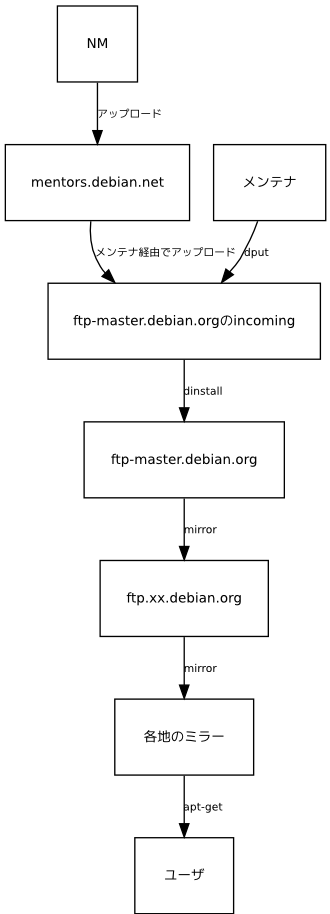
\includegraphics[height=0.8\vsize]{image200801/maint-package.png}

 \subsection{開発者のパッケージングの契機}

開発者がパッケージを作成するタイミングとはどういうものがあるでしょうか。
簡単にいうと三つあります:

 \begin{itemize}
 \item Debianに存在しない全く新しいパッケージ(ITPからの一連の流れをふむ)
 \item Debianにすでに存在しているパッケージの新しいアップストリームバージョンがリリースされた
 \item Debianにすでに存在しているパッケージにユーザがバグ報告をし、
       BTSに登録されたバグ報告の内容に対応するにはパッケージの修正が必要
       になった
  \item 依存関係が更新されたから更新
 \end{itemize}

\begin{figure}[h]
%inkscape --export-text-to-path --export-eps=devel-logic-i.eps devel-logic-i.svg 
 \begin{center}
  \includegraphics[width=0.8\hsize]{image200801/devel-logic-i.eps}
 \end{center} 
 \caption{開発者のロジックの流れ}
\end{figure}

 \subsection{作業の流れ}
 \subsubsection{アップストリームの取得}

新しいソースパッケージを取得します。tar.gz で公開されていればそのまま使
えます。tar.bz2 であったり、よくわからないアーカイブフォーマットだったり、
gitレポジトリでしか公開されていなかったりするので、それなりに加工します。

最初は適当に取得するわけですが、二回目移行はスクリプトで自動化して取得す
るようにします。watch という仕組みがあり、 uscan / uupdate コマンドで新しいバージョ
ンをダウンロードしてきてDebianパッケージ用のパッチを適用することができま
す。

\begin{figure}[h]
 \begin{commandline}
 version=3

 http://ftp.imendio.com/pub/imendio/giggle/src/giggle-(.*)\.tar\.gz

 \end{commandline}
\label{watchfile}
\caption{giggle パッケージの debian/watch ファイル}
\end{figure}


\subsubsection{パッケージング}

二度めからは差分の適用などで対応できるのですが、最初の新規パッケージの場
合はITPなどの処理を必要とします。また、新規にパッケージを作成するので、
なんらかのテンプレートパッケージから debian/ ディレクトリを取得してきて
修正するか、 dh\_make コマンドを利用してテンプレートを作成します。

この段階で debhelper を利用するのか、 cdbs を利用するのかの選択を迫られ
ます。cdbs は debhelper より新しい仕組みですが、2003年の登場から5年もたっ
ているのでそろそろこなれています。簡単なパッケージであれば cdbs を利用す
ればよいでしょう。現状の cdbs のフレームワークで不具合があるような場合で
あれば debhelper で詳細に設定するのがよいでしょう。

\begin{commandline}
$ dh_make 

Type of package: single binary, multiple binary, library, kernel module or cdbs?
 [s/m/l/k/b] b

Maintainer name : Junichi Uekawa
Email-Address   : dancer@debian.org 
Date            : Fri, 18 Jan 2008 22:22:51 +0900
Package Name    : tttt
Version         : 2.2
License         : blank
Type of Package : cdbs
Hit <enter> to confirm: 
Could not find tttt_2.2.orig.tar.gz
Either specify an alternate file to use with -f,
or add --createorig to create one.
[22:22:55]coreduo:tttt-2.2> 
\end{commandline}

 \subsubsection{BTSとの対応}

BTSに登録されているバグ報告に対してメールで対応したりします。
報告されている不具合をちゃんと修正してみたりします。

BTSは閲覧はWebでできますが、制御はWebではできません。BTSはメールで命令を
直接うって制御できます。メールコマンドはすぐに忘れてしまうので、
\url{/usr/share/doc/debian/bug-*} あたりを参照しながら作業します。BTSの
操作に便利なツールがいくつかあるので、そちらを利用することをおすすめしま
す。

\begin{itemize}
 \item  reportbug-ng 
 \item  reportbug
 \item  dpkg-dev-el 
\end{itemize}

 \subsubsection{ChangeLog の管理}

パッケージの新しいバージョンを作成する場合には、debian/changelog に対応
内容を記述します。
ここで活用できるツールには次があります。

\begin{itemize}
 \item devscripts の dch
 \item dpkg-dev-el の debian-changelog.el
 \item vim の debchangelog 
\end{itemize}

バージョン番号を自動で増加させてくれたり、いろいろなエントリーの補完など
をしてくれます。BTSを参照して修正されたバグのタイトルから ChangeLog のエ
ントリを生成してくれたりもします。

\begin{commandline}
pbuilder (0.177) unstable; urgency=low

  [ Loic Minier ]
  * Run apt-get autoremove after upgrade.

  [ Junichi Uekawa ]
  * python-apt/gdebi based pbuilder-satisfydepends-gdebi (closes:
    #453388)
  * Fix devpts mount permissions (closes: #453862)
  * Document pbuilder-satisfydepends-gebi in manpage

 -- Junichi Uekawa <dancer@debian.org>  Wed, 26 Dec 2007 20:53:24 +0900

\end{commandline}

\subsubsection{ビルド・テスト}

debian/以下のファイルを微調整して、パッケージをビルドします。
dpkg-buildpackage を直接呼び出してもよいですが、devscripts パッケージの
debuildコマンドを利用すればよいでしょう。

lintian / linda で生成されたパッケージにあきらかな間違いがないことを確認
します。

debc, debdiff で生成されたパッケージにあきらかな間違いや意図しない大きな
変化がないことを確認します。

debi でパッケージをインストールして正常に動作することを確認します。

pbuilder でビルドしてみて問題ないことを確認します。

pbuilder のテストスクリプトpbuilder-test を利用してインストール・アンイ
ンストール・アップグレードの試験をしてみるとさらによいでしょう。

 \subsubsection{アップロード}

署名してアップロードします。dpkg-buildpackage コマンドを利用してパッケー
ジをビルドすると自動でgpgで署名することになります。あとで署名しなおす場
合には、 debsign を利用します。

アップロードは dput コマンドを利用します。

 \subsection{非公式パッケージレポジトリの作成方法}

 テスト用に非公式のパッケージレポジトリを準備すると便利です。

 Packages.gz ファイルなどを生成してHTTP経由でアクセスできるようにしておく
 と、ユーザが /etc/apt/sources.list に追記することで apt を利用してパッケー
 ジが取得できるようになります。

 \begin{itemize}
  \item dpkg-scanpackages / dpkg-scansources を直接利用する方法。
  \item apt-ftparchive を利用する方法。
  \item mini-dinstall を利用する方法。
  \item apt-move を利用する方法。
  \item debarchiver
  \item reprepro
  \item dak
 \end{itemize}

2007年9月号で apt-ftparchive が紹介されていたので再掲します。

\subsubsection{apt-ftparchive}
 Sources.gz / Packages.gz などのパッケージ情報用ファイルを作成するためのツール。
 自分で作ったパッケージを apt-line として公開したいときに使います。
\begin{commandline}
  % apt-ftparchive packages . | gzip -9 > Packages.gz 
  % apt-ftparchive sources . | gzip -9 > Sources.gz
  % apt-ftparchive release . > Release 
\end{commandline}

\subsubsection{apt-sortpkgs}
 Packages ファイル および Sources ファイルをソートします。apt-ftparchive で作成したものはソート
 されていなかったりするので、アルファベット順にソートするときに使います。
\begin{commandline}
 % apt-sortpkgs Packages > Packages.sort
\end{commandline} 

 \subsection{参考文献}

 必読の文献として、以下があります。一通り読んだ後は、パッケージとしてイン
 ストールしておき、手元で検索できるようにしておくと便利です。sid を利用
 しているのであれば、パッケージとしてインストールしておくと最新版に勝手に
 更新されるため、便利です。

 内容に誤記などがあれば、ぜひBTSにバグ報告を登録してください。

 \begin{itemize}
 \item debian-policy: Debian Policy Manual。
       パッケージの準拠すべきルールが文書化されています。
 \item developers-reference: Developers Reference。
       
 \item doc-debian: Debian Project Documentation。 BTSのメールインタフェー
       スなどの文書がある。
 \item maint-guide: Debian New Maintainer's guide。
       New Maintainerとして知るべきマナーのようなものが文書化されていま
       す。
 \end{itemize}


%\end{multicols}

\clearpage

%\printindex

\cleartooddpage

\vspace*{15cm}
\hrule
\vspace{2mm}

\includegraphics[width=2cm]{image200502/openlogo-nd.eps}
\noindent \Large \bf Debian 勉強会資料\\ \\
\noindent \normalfont \debmtgyear{}年\debmtgmonth{}月\debmtgdate{}日 \hspace{5mm}  初版第1刷発行\\
\noindent \normalfont 東京エリア Debian 勉強会 (編集・印刷・発行)\\
\hrule


\end{document}
